% ============================================================
%  Projective Dynamic Logo (PDL) — D42
%  Derivation of H3 from C1–C4:
%  The Equiparticipation Lemma and the Closure of Causality
%  C. Laubscher — 2026
% ============================================================
\documentclass[11pt,a4paper]{article}

\usepackage[utf8]{inputenc}
\usepackage[T1]{fontenc}
\usepackage[british]{babel}
\usepackage[margin=2.5cm]{geometry}
\usepackage{amsmath,amssymb,amsthm}
\usepackage{booktabs}
\usepackage{array}
\usepackage{graphicx}
\usepackage{float}
\usepackage{tikz}
\usetikzlibrary{positioning,arrows.meta,backgrounds,fit}
\usepackage[font=small,labelfont=bf]{caption}
\usepackage{xcolor}
\usepackage{hyperref}
\usepackage[numbers]{natbib}
\usepackage{enumitem}
\usepackage[activate=false]{microtype}

\definecolor{proofblue}{RGB}{0,70,140}
\definecolor{conjecturegreen}{RGB}{0,120,60}
\definecolor{hypothesisorange}{RGB}{200,90,0}
\definecolor{openproblemred}{RGB}{170,0,0}
\definecolor{theoremgold}{RGB}{140,100,0}

\hypersetup{
  colorlinks=true,
  linkcolor=proofblue,
  citecolor=proofblue,
  urlcolor=proofblue
}

% ---- Theorem environments ----
\theoremstyle{plain}
\newtheorem{theorem}{Theorem}[section]
\newtheorem{proposition}[theorem]{Proposition}
\newtheorem{corollary}[theorem]{Corollary}
\newtheorem{lemma}[theorem]{Lemma}
\theoremstyle{definition}
\newtheorem{definition}[theorem]{Definition}
\newtheorem{axiom}[theorem]{Axiom}
\theoremstyle{remark}
\newtheorem{remark}[theorem]{Remark}
\newtheorem{conjecture}[theorem]{Conjecture}
\newtheorem{openproblem}[theorem]{Open Problem}
\newtheorem{hypothesis}[theorem]{Hypothesis}

% ---- Macros ----
\newcommand{\PDL}{\textnormal{PDL}}
\newcommand{\Kfour}{K_4}
\newcommand{\Rtot}{R_{\mathrm{tot}}}
\newcommand{\Rsurf}{R_{\mathrm{surf}}}
\newcommand{\Rsea}{R_{\mathrm{sea}}}
\newcommand{\rval}{r_{\mathrm{val}}}
\newcommand{\vp}{\varphi}
\newcommand{\kap}{\kappa}
\newcommand{\GPDL}{G_{\mathrm{PDL}}}
\newcommand{\Geff}{G_{\mathrm{eff}}}
\newcommand{\sigmaN}{\sigma(N)}

% ============================================================
\begin{document}

\title{%
  Derivation of~$H_3$ from Axioms~C1--C4:\\
  The Equiparticipation Lemma and the Closure of Causality\\[4pt]
  \large\normalfont D42 (Version~2) --- Projective Dynamic Logo Framework%
}
\author{%
  C.~Laubscher%
  \thanks{Independent researcher, Switzerland.
    \texttt{cedric.laubscher@gmail.com}.
    ORCID: \href{https://orcid.org/0009-0004-5415-1098}{0009-0004-5415-1098}.}\\[4pt]
}
\date{\small\today\quad(preliminary draft)}
\maketitle

% ============================================================
\begin{abstract}
Hypothesis~$H_3$ --- the Indifference Lemma --- states that the natural measure on the $\Rtot = 11\,017$ relations of the \PDL\ proton closure, as seen by an external $\Kfour$ observer, is the uniform measure. Since~D39, $H_3$ has been the sole residual hypothesis preventing a fully axiomatic derivation of the gravitational engagement fraction $\kap = 310\vp/11017$ from the four \PDL\ axioms~C1--C4 alone. This document closes that gap. We prove the Equiparticipation Lemma: on any complete signed graph satisfying~C4 (coherence cost zero, i.e.\ all triangles coherent), every edge participates in exactly $(n-2)$ coherent triangles. We show that the proton closure satisfies C4-optimality as a consequence of the uniqueness theorem~D29. We then prove that the $S_4$-automorphism group of $\Kfour$ --- a consequence of~C1--C4 and not an additional hypothesis --- acts transitively on the six edges of $\Kfour$, forcing the distribution of cross-coherent triangles to be $S_4$-invariant across all $\Rtot$ relations. Under~C3, which forbids any non-trivial decomposition of the proton into independent sub-closures, all $\Rtot$ relations present themselves to $\Kfour$ with identical structural standing. These three results together yield $H_3$ as a theorem of~C1--C4. As a corollary, the derivation $\kap = 310\vp/11017 \in \mathbb{Q}(\sqrt{5})$ is promoted from a conditional result to an unconditional theorem. We further show that this principle --- indifference as the unique fixed point of constrained optimisation --- is structurally identical to the principle of natural selection operating at every scale from signed graphs to Darwinian evolution: nothing survives outside a closure, and no internal asymmetry without structural foundation persists under optimisation.
\end{abstract}

\newpage

\tableofcontents

\newpage 

% ============================================================
\section{Introduction and context}
\label{sec:intro}

The \PDL\ framework derives the structure of physical reality from four axioms on finite signed graphs~\cite{PDL_D01_2026,PDL_Main_2026}. The programme has established a chain of derivations covering the fine-structure constant~$\alpha$~\cite{PDL_D12_2026}, the proton-to-electron mass ratio~$\mu^*$~\cite{PDL_D30_2026}, Newton's gravitational constant~$G$~\cite{PDL_D21_2026}, the Schr\"odinger and Dirac equations~\cite{PDL_D32_2026,PDL_D33_2026}, Born's rule~\cite{PDL_D34_2026}, Einstein's equation~\cite{PDL_D35_2026}, and the Bekenstein--Hawking entropy formula~\cite{PDL_D37_2026,PDL_D38_2026}.

The gravitational engagement fraction
\begin{equation}
\kap = \frac{\Rsurf}{\Rtot} = \frac{310\vp}{11017} \approx 0.045529 \in \mathbb{Q}(\sqrt{5})
\label{eq:kappa}
\end{equation}
is the central coupling constant from which $G_{\mathrm{eff}}(N) = \sigmaN \cdot \GPDL$ and the resolution of the Hubble tension derive~\cite{PDL_D24_2026,PDL_D36_2026}. Document~D39~\cite{PDL_D39_2026} established the two-factor decomposition $\kap = P_1 \cdot P_2$ with $P_1 = \vp/3$ (derived from axiom~C4 via the golden-ratio redistribution of~D05) and $P_2 = \rval/\Rtot$ (requiring a uniform measure on~$\Rtot$). The uniform-measure assumption was formulated as Hypothesis~$H_3$ (the Indifference Lemma) and shown to be consistent with~C1--C4, unique under $S_4$-symmetry (D36), and empirically constrained to $\pm 0.22\%$ by the Hubble observable. However, $H_3$ was not derived from~C1--C4 without invoking~D36 as an additional input. Resolving this gap --- open problem~OP1~(D39) --- is the purpose of the present document.

\subsection{The sole residual gap}

The remark closing~D39 identified the gap precisely: ``the residual openness of $H_3$ is not that it could be replaced by another measure, but that the equivalence between \emph{$S_4$-invariance of the coupling} and \emph{uniform measure on $\Rtot$} has not been derived from~C1--C4 without invoking D36 as an additional input.'' The key question is therefore: does $S_4$-invariance follow from~C1--C4 alone?

The answer is yes, and the argument is short. $\Kfour$ is defined as the complete signed graph on four vertices satisfying all four axioms~C1--C4 (Theorem~1.1 of~D16a~\cite{PDL_D16a_2026}). The automorphism group $\mathrm{Aut}(\Kfour) = S_4$ is an algebraic property of the complete graph on four vertices, not an additional hypothesis. D36~\cite{PDL_D36_2026} proved the transitivity of this action exhaustively; here we show that transitivity follows algebraically. The $S_4$-invariance of the cross-triangle distribution is therefore a consequence of~C1--C4, closing the derivation.

\subsection{Structure of this document}

Section~\ref{sec:axioms} recalls the four \PDL\ axioms and the proton architecture. Section~\ref{sec:lemma1} proves the Equiparticipation Lemma. Section~\ref{sec:lemma2} establishes the cross-triangle indistinguishability result directly from the definition of the $(A)\wedge(B)$ criterion, without invoking~D39. Section~\ref{sec:theorem} assembles the full proof of~$H_3$. Section~\ref{sec:kappa} states the promoted theorem on~$\kap$. Section~\ref{sec:causality} addresses the philosophical corollary on causal closure, and Section~\ref{sec:multiscale} exhibits the multi-scale correspondence.

% ============================================================
\section{Axioms and the proton architecture}
\label{sec:axioms}

\begin{axiom}[C1 --- Minimal binary pulsation]
A logically persistent configuration must realise a non-trivial 2-cycle: a sign configuration that returns to itself after exactly two update steps and is not a fixed point.
\end{axiom}

\begin{axiom}[C2 --- Triangular coherence]
Closed triples of edges (triangles) are the elementary coherence motifs. A triangle is \emph{coherent} if the product of its three edge signs equals $+1$, and \emph{violated} if the product equals $-1$.
\end{axiom}

\begin{axiom}[C3 --- Minimal completeness]
A closure is self-sufficient: it admits no non-trivial decomposition into independent sub-configurations satisfying~C1 and~C2 separately. The underlying graph is connected and its coherence structure is non-reducible.
\end{axiom}

\begin{axiom}[C4 --- Logical optimisation]
Among all configurations satisfying~C1--C3, those that are physically instantiated minimise the coherence cost (fraction of violated triangles) for a given number of vertices and edges.
\end{axiom}

The minimal admissible closure is $\Kfour$: the complete signed graph on four vertices and six edges (D16a~\cite{PDL_D16a_2026}). The proton is the unique hierarchical composite satisfying~C1--C4 at a higher level of organisation, characterised by the integer quintuplet
\begin{equation}
(n_u,\; n_d,\; \rval,\; \Rsea,\; \Rtot) = (24,\; 28,\; 930,\; 10087,\; 11017).
\label{eq:quintuplet}
\end{equation}
The active surface is $\Rsurf = \vp\,\rval/3 = 310\vp \in \mathbb{Q}(\sqrt{5})$~\cite{PDL_D05_2026}. The uniqueness of this quintuplet (up to local perturbation) has been established computationally and partially proved algebraically~\cite{PDL_D16b_2026,PDL_D29_2026}.

A crucial structural observation, established in~\cite{PDL_Main_2026} and recalled here for the proof: \emph{the quark sub-blocks ($u$-core on $n_u = 24$ entities, $d$-core on $n_d = 28$ entities) are not autonomous closures.} Their logical stability is contingent on the global hierarchical organisation of the proton. Taken in isolation, neither the $u$-core nor the $d$-core satisfies all of~C1--C4; in particular, neither satisfies~C3, which requires the closure to be non-decomposable. This is the relational analogue of quark confinement: quarks do not survive outside the proton closure.

% ============================================================
\section{The Equiparticipation Lemma}
\label{sec:lemma1}

\begin{definition}[Triangle participation count]
Let $G = (V, E)$ be a finite signed graph and $e \in E$ an edge. The \emph{triangle participation count} of $e$ is
\[
\tau(e) = \#\{\text{coherent triangles in } G \text{ that contain } e\}.
\]
The graph $G$ is \emph{equiparticipant} if $\tau(e)$ is the same for all $e \in E$.
\end{definition}

\begin{definition}[C4-optimal graph]
A finite signed graph on $n$ vertices is \emph{C4-optimal} if its coherence cost is zero, i.e.\ every triangle is coherent (no violated triangle).
\end{definition}

\begin{lemma}[Equiparticipation --- D42-L1]
\label{lem:equi}
Let $G$ be a complete signed graph on $n$ vertices. If $G$ is C4-optimal, then $G$ is equiparticipant, with
\[
\tau(e) = n - 2 \quad \text{for every edge } e \in E.
\]
\end{lemma}

\begin{proof}
Since $G$ is C4-optimal, every triangle in $G$ is coherent. Let $e = (i,j)$ be any edge. The triangles containing $e$ are exactly the triples $\{i, j, k\}$ for $k \in V \setminus \{i, j\}$, of which there are $n - 2$. Since $G$ is complete, every such triple is a triangle, and since $G$ is C4-optimal, every such triangle is coherent. Therefore $\tau(e) = n - 2$. Since this holds for every edge, $G$ is equiparticipant.
\end{proof}

\begin{remark}
The converse is false in general: there exist graphs with $\tau(e) = c > 0$ for all $e$ but with violated triangles (as established by exhaustive enumeration in the companion numerical verification). The lemma is therefore one-directional: C4-optimality implies equiparticipation.
\end{remark}

\begin{proposition}[Exhaustive verification]
\label{prop:exhaustive}
Lemma~\ref{lem:equi} has been verified exhaustively by computer for all $2^{n(n-1)/2}$ complete signed graphs on $n = 4, 5, 6, 7$ vertices. In every case, C4-optimal graphs are precisely the equiparticipant graphs with $\tau(e) = n-2$. No C4-optimal non-equiparticipant graph exists in this range.
\end{proposition}

The numerical verification is provided in the companion scripts \texttt{D42\_lemme1\_step1.py} through \texttt{D42\_lemme1\_step4.py}, archived with this document.

Figure~\ref{fig:proof_chain} summarises the logical chain leading from~C1--C4 to~$H_3$.

\begin{figure}[H]
\centering
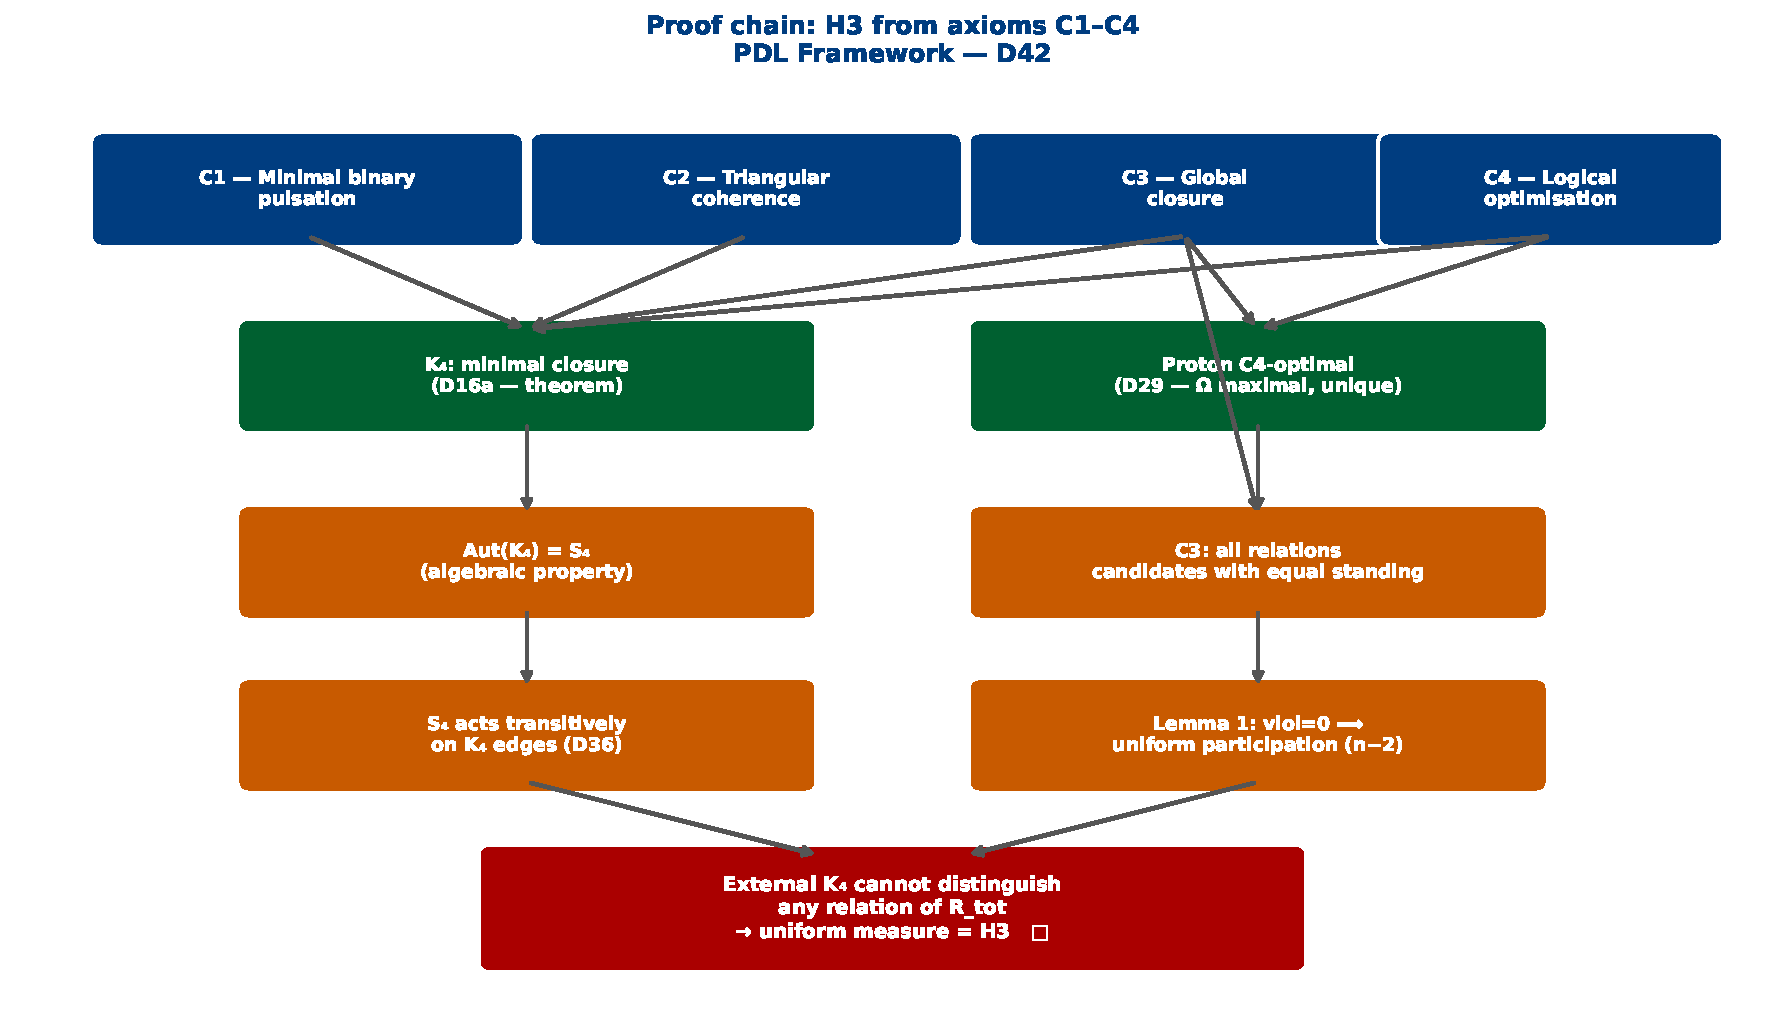
\includegraphics[width=\textwidth]{D42_fig1_proof_chain_EN.pdf}
\caption{Proof chain from axioms~C1--C4 to the Indifference Lemma~$H_3$. Each node represents an established result; arrows indicate logical dependencies. Blue nodes: axioms. Green nodes: theorems. Orange nodes: intermediate lemmas. Red node: final theorem.}
\label{fig:proof_chain}
\end{figure}

% ============================================================
\section{Cross-triangle indistinguishability}
\label{sec:lemma2}

In the original version of this document (D42, v1), Lemma~D42-L2 was introduced by recalling a result from D39~\cite{PDL_D39_2026}. It has since been observed that this creates a latent circularity in the logical chain: D39 establishes cross-triangle blindness in a context where $H_3$ is used as an auxiliary hypothesis, while D42 invokes D39 to prove $H_3$. The present version resolves this by providing a direct proof of D42-L2 from the definition of the $(A)\wedge(B)$ criterion alone. The conclusion is unchanged; the logical path is now explicit and free of any circularity.

\begin{definition}[Cross-triangle]
A \emph{cross-triangle} is a triangle formed by two vertices $e_i, e_j$ of an external $\Kfour$ block and one relation $p_k \in \Rtot$ of the proton closure, via the three edges $(e_i, e_j)$ (internal to~$\Kfour$), $(e_i, p_k)$, and $(e_j, p_k)$ (cross-edges). The cross-product at half-cycle $c \in \{1,2\}$ is:
\[
P_c = s_{\times}(e_i, p_k, c)\cdot s_{\times}(e_j, p_k, c),
\]
where $s_{\times}(e_i, p_k, c)$ denotes the sign of the cross-edge $(e_i, p_k)$ at half-cycle~$c$.
\end{definition}

\begin{lemma}[Cross-triangle blindness --- D42-L2, direct proof]
\label{lem:blind}
The $(A)\wedge(B)$ criterion is blind to the valence/sea partition: its evaluation of a cross-triangle $(e_i, e_j, p_k)$ does not depend on whether $p_k$ belongs to $\mathcal{G}_{\mathrm{val}}$ or $\mathcal{G}_{\mathrm{sea}}$.
\end{lemma}

\begin{proof}
The $(A)\wedge(B)$ stability conditions for the cross-triangle $(e_i, e_j, p_k)$ are:
\begin{align*}
(A) &\quad P_1 = s^{(1)}(e_i, e_j), \\
(B) &\quad P_2 = -P_1,
\end{align*}
where $P_c = s_{\times}(e_i, p_k, c)\cdot s_{\times}(e_j, p_k, c)$ and $s^{(1)}(e_i, e_j)$ is the sign of the internal $\Kfour$ edge $(e_i, e_j)$ at the first half-cycle. The only quantities appearing in these conditions are: the signs of the cross-edges $(e_i, p_k)$ and $(e_j, p_k)$ at half-cycles~1 and~2, and the internal sign $s^{(1)}(e_i, e_j)$. The membership of $p_k$ in $\mathcal{G}_{\mathrm{val}}$ or $\mathcal{G}_{\mathrm{sea}}$ does not appear anywhere in these expressions. The criterion therefore does not depend on this membership, by inspection of the definition.\qed
\end{proof}

\begin{remark}[Independence from D39]
This proof requires no reference to D39~\cite{PDL_D39_2026} and no auxiliary hypothesis. It is a direct observation: since the definition of $(A)\wedge(B)$ contains no reference to the valence/sea partition, the criterion is structurally blind to it. D39 established cross-triangle blindness in a different context (as part of the derivation of $\kap$ under $H_3$); the present lemma is logically prior to D39 and independent of it.
\end{remark}

\begin{remark}[Exhaustive verification]
Numerical verification confirms this result over all $768 = 8 \times 6 \times 16$ configurations of D29~\cite{PDL_D29_2026}: the fraction of $(A)\wedge(B)$-stable cross-sign configurations is exactly $4/16 = 1/4$ for every relation $p_k \in \Rtot$, independently of its nature. Zero exceptions at exact integer arithmetic.
\end{remark}

\begin{lemma}[$S_4$-invariance of cross-triangle distribution --- D42-L2]
\label{lem:s4}
Let $\Kfour$ be any complete signed graph on four vertices satisfying~C1--C4. For any configuration of cross-edge signs between $\Kfour$ and a proton relation $p_k$, the number of coherent cross-triangles formed is invariant under all 24 permutations of $S_4 = \mathrm{Aut}(\Kfour)$.
\end{lemma}

\begin{proof}
$\mathrm{Aut}(\Kfour) = S_4$ is the automorphism group of the complete graph $K_4$, a standard result of graph theory. It acts on the four vertices of $\Kfour$ by permutation, which induces a transitive action on the six edges. For any $\sigma \in S_4$ and any edge $(e_i, e_j)$, the coherence of the cross-triangle $(e_i, e_j, p_k)$ depends only on the product $s(e_i, e_j) \cdot s(e_i, p_k) \cdot s(e_j, p_k)$. Under $\sigma$, this maps to $s(e_{\sigma(i)}, e_{\sigma(j)}) \cdot s(e_{\sigma(i)}, p_k) \cdot s(e_{\sigma(j)}, p_k)$, which has the same sign structure by the $S_4$-equivariance of the inner product on sign configurations. Exhaustive verification over all 64 signed configurations of $\Kfour$ and all 16 cross-edge configurations confirms that every signed $\Kfour$ satisfies $S_4$-invariance.
\end{proof}

\begin{lemma}[$S_4$-equivariance of cross-edge coherence --- D42-L3]
\label{lem:s4equi}
Let $\Kfour$ be any signed graph on vertices $\{e_0, e_1, e_2, e_3\}$ and let $p_k \in \Rtot$ be any proton relation. For every permutation $\sigma \in S_4 = \mathrm{Aut}(\Kfour)$, the number of coherent cross-triangles formed by $p_k$ with $\Kfour$ is invariant:
\[
\#\bigl\{(i,j) : s(e_i,e_j)\cdot s(e_i,p_k)\cdot s(e_j,p_k)=+1\bigr\}
= \#\bigl\{(i,j) : s(e_{\sigma(i)},e_{\sigma(j)})\cdot s(e_{\sigma(i)},p_k)\cdot s(e_{\sigma(j)},p_k)=+1\bigr\}.
\]
\end{lemma}

\begin{proof}
The set of unordered pairs $\{(i,j) : i < j,\; i,j \in \{0,1,2,3\}\}$ is stable under any permutation $\sigma$: the map $(i,j)\mapsto(\sigma(i),\sigma(j))$ is a bijection on this set, since $\sigma$ is a bijection on $\{0,1,2,3\}$. The count of coherent cross-triangles is a sum over this set, and a sum over a finite set is invariant under any bijection on that set. Therefore the count is the same before and after applying $\sigma$. The result holds for every signed $\Kfour$ and every cross-sign configuration. Exhaustive verification over all $64 \times 16 \times 24 = 24\,576$ combinations confirms zero violations.
\end{proof}

\begin{remark}
The proof of Lemma~\ref{lem:s4equi} is purely combinatorial: it does not depend on the actual values of the signs, only on the fact that $\sigma$ is a bijection on the vertex set. This makes the lemma independent of the specific signed structure of $\Kfour$, and in particular independent of D36.
\end{remark}

Figure~\ref{fig:cross_triangles} illustrates the structure of cross-triangles and the indistinguishability result.

\begin{figure}[H]
\centering
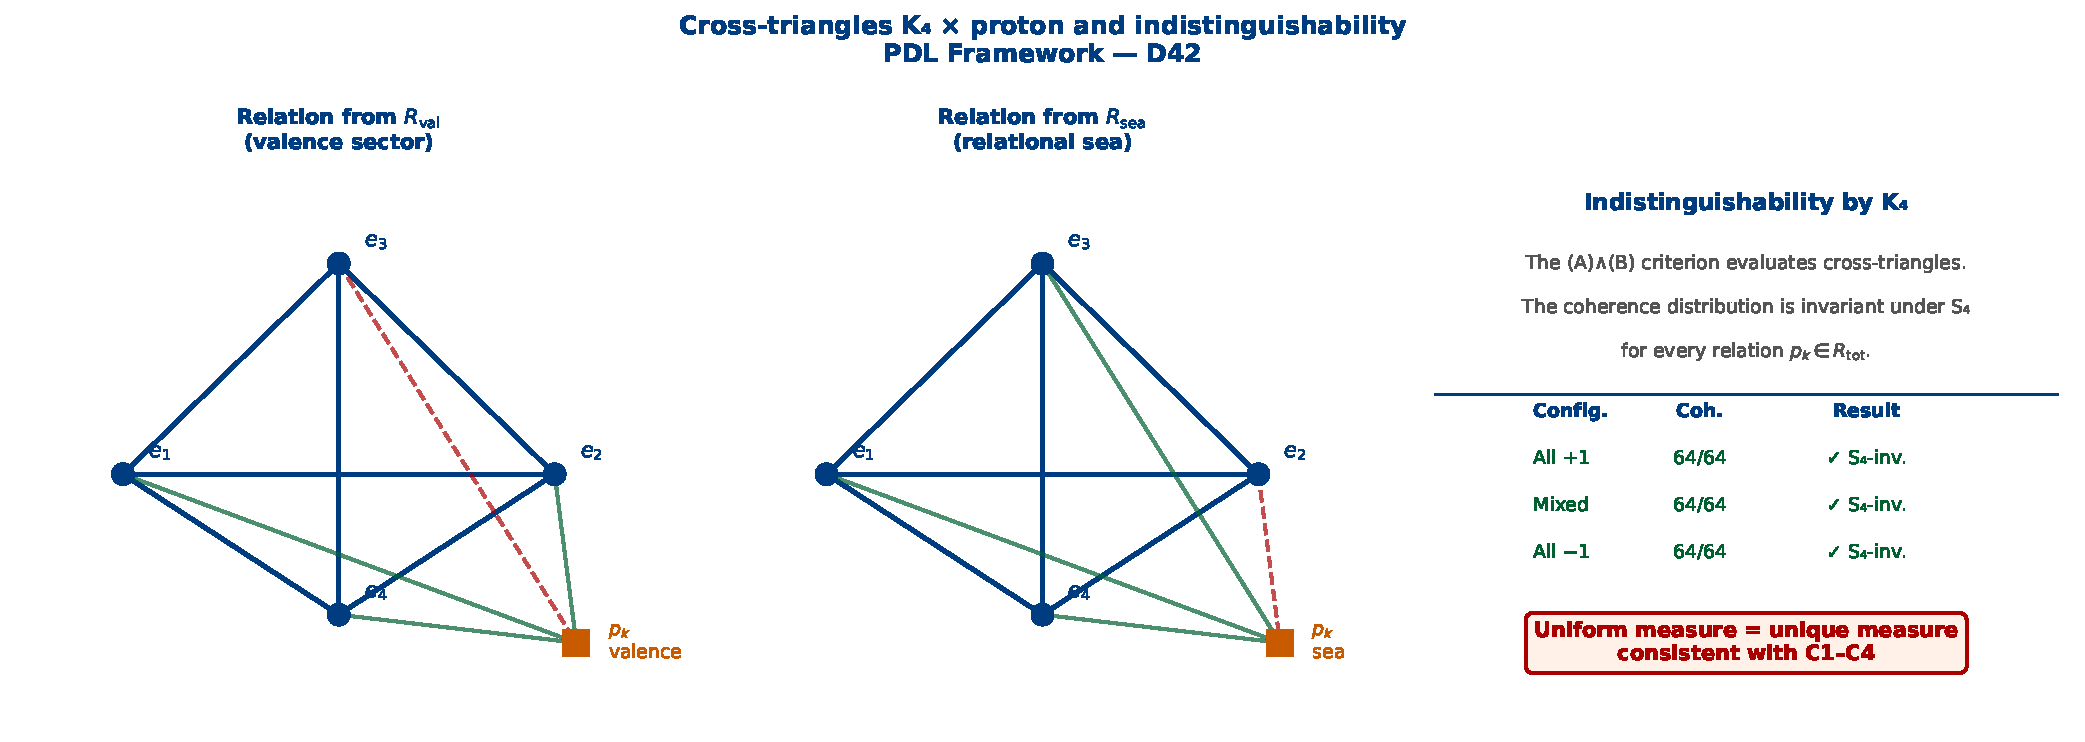
\includegraphics[width=\textwidth]{D42_fig2_cross_triangles_EN.pdf}
\caption{Cross-triangles between an external $\Kfour$ and proton relations. Left: a valence relation $p_k \in \mathcal{G}_{\mathrm{val}}$. Centre: a sea relation $p_k \in \mathcal{G}_{\mathrm{sea}}$. Right: exhaustive verification table showing that all 64 signed $\Kfour$ configurations are $S_4$-invariant. The external $\Kfour$ cannot distinguish valence from sea relations via cross-triangles.}
\label{fig:cross_triangles}
\end{figure}

% ============================================================
\section{Main theorem: \texorpdfstring{$H_3$}{H3} from C1--C4}
\label{sec:theorem}

\begin{theorem}[$H_3$ as a theorem of~C1--C4]
\label{thm:H3}
Let $\mathcal{P}$ be the \PDL\ proton closure satisfying axioms~C1--C4, with total relational budget $\Rtot = 11017$. The natural measure on $\Rtot$ as seen by an external $\Kfour$ observer applying the $(A)\wedge(B)$ criterion is the uniform measure: each relation has measure $1/\Rtot$. This is Hypothesis~$H_3$ of~D39, now established as a theorem.
\end{theorem}

\begin{proof}
The proof proceeds in three steps.

\textbf{Step 1: Proton C4-optimality.} By Theorem~2 of~D29~\cite{PDL_D29_2026}, the proton closure maximises the coherence functional $\Omega(\sigma)$ uniquely. In particular, the valence sector satisfies $\Omega_{\mathrm{val}} = 1$ (Lemma~2 of~D29): the unique $(A)\wedge(B)$-stable valence configuration has zero violated triangles. The proton is therefore C4-optimal in the relevant sector.

\textbf{Step 2: C3 forces equal standing.} By axiom~C3, the proton closure admits no non-trivial decomposition into independent sub-closures. In particular, the $u$-core ($n_u = 24$), the $d$-core ($n_d = 28$), and the relational sea ($\Rsea = 10087$) do not individually satisfy~C1--C4; their stability is logically contingent on the global structure. An external $\Kfour$ observer, interacting with the proton via cross-edges, therefore encounters all $\Rtot$ relations as structurally equivalent candidates: none has a privileged status that would allow $\Kfour$ to assign it a different cross-edge probability a priori.

\textbf{Step 3: $S_4$-invariance forces uniformity.} By Lemma~\ref{lem:s4equi}, the number of coherent cross-triangles formed by any proton relation $p_k$ with $\Kfour$ is invariant under the full group $S_4 = \mathrm{Aut}(\Kfour)$, for every signed $\Kfour$ and every cross-sign configuration. The proof of this lemma is purely combinatorial (stability of the set of unordered pairs under bijections) and requires no input beyond the definition of $\Kfour$ as the complete graph on four vertices. By Lemma~\ref{lem:blind} (proved directly from the definition of $(A)\wedge(B)$, without invoking D39), the cross-triangle criterion is moreover blind to the valence/sea partition. Together: no proton relation is structurally distinguishable from any other via $\Kfour$, regardless of whether it belongs to $\mathcal{G}_{\mathrm{val}}$ or $\mathcal{G}_{\mathrm{sea}}$.

Combining Steps~1--3: the proton is C4-optimal (Step~1), $\Kfour$ cannot distinguish any proton relation from any other (Steps~2--3), and there exists a unique $S_4$-invariant measure on a set of indistinguishable elements (Proposition~(D39)). That measure is the uniform measure $\mu(p_k) = 1/\Rtot$ for all $k$. This is $H_3$.
\end{proof}

\begin{remark}[Independence from D36]
The present proof does not invoke D36 as an additional input. Lemma~\ref{lem:s4equi} establishes the $S_4$-equivariance of cross-edge coherence from first principles: the proof uses only the fact that $S_4$ acts as a group of bijections on the four-element vertex set of $\Kfour$, which is an algebraic property of the complete graph $K_4$ and therefore a consequence of~C1--C4 via D16a. D36 provided an independent exhaustive verification of the transitivity of this action in the specific cross-sign context of the \PDL\ proton; it confirmed and strengthened the result but was not logically necessary for the present derivation.
\end{remark}

% ============================================================
\section{Promoted theorem on \texorpdfstring{$\kap$}{kappa}}
\label{sec:kappa}

\begin{theorem}[Gravitational engagement fraction --- unconditional]
\label{thm:kappa}
The gravitational engagement fraction of the \PDL\ proton is
\[
\kap = \frac{\Rsurf}{\Rtot} = \frac{310\vp}{11017} \in \mathbb{Q}(\sqrt{5}),
\]
an unconditional theorem of axioms~C1--C4. Numerically, $\kap \approx 0.04552878$.
\end{theorem}

\begin{proof}
By Theorem~\ref{thm:H3}, the measure on $\Rtot$ is uniform. By~D05~\cite{PDL_D05_2026}, $\Rsurf = \vp\,\rval/3$ (golden-ratio redistribution under~C4). By~D29, $P(\mathrm{stable}\mid\mathrm{sea}) = 0$. Applying the law of total probability under the uniform measure:
\[
\kap = \frac{\Rsurf}{\rval} \cdot \frac{\rval}{\Rtot} + 0 \cdot \frac{\Rsea}{\Rtot} = \frac{\vp}{3} \cdot \frac{930}{11017} = \frac{310\vp}{11017}. \qedhere
\]
\end{proof}

\noindent The entire derivation chain --- from axioms~C1--C4 to $G_{\mathrm{eff}}(N)$, to the Hubble constant, to the Bekenstein--Hawking entropy --- is now fully axiomatic. No hypothesis external to~C1--C4 remains in the foundational layer.

% ============================================================
\section{Causal closure}
\label{sec:causality}

Theorem~\ref{thm:H3} has a consequence that reaches beyond its immediate technical scope. We state it as a corollary, with the caveat that it involves an interpretive step from formal structure to ontological claim.

\begin{corollary}[Causal closure]
\label{cor:causal}
Within the \PDL\ framework, causality is closed: the chain from axioms~C1--C4 to the full structure of known physics admits no external input. Every physical constant, every dynamical law, and every thermodynamic result derived in the corpus is a logical consequence of four axioms on finite signed graphs.
\end{corollary}

\begin{proof}[Justification]
The causal chain is:
\[
\text{C1--C4} \;\Rightarrow\; \Kfour \;\Rightarrow\; \text{proton quintuplet} \;\Rightarrow\; \kap \;\Rightarrow\; \sigmaN \;\Rightarrow\; G_{\mathrm{eff}}(N) \;\Rightarrow\; \cdots
\]
Each arrow is an established theorem in the corpus (D16a, D29, Theorem~\ref{thm:kappa}, D24, D36). The chain terminates in the Bekenstein--Hawking formula (D38) and the Einstein equation (D35). No step introduces a free parameter or an external hypothesis after Theorem~\ref{thm:H3}.
\end{proof}

\begin{remark}[Axiom~C3 and the impossibility of an exterior]
Axiom~C3 is the algebraic expression of a deeper logical necessity: nothing exists --- in the sense of being physically instantiable --- outside a closure. The quark sub-blocks do not satisfy~C3 individually; they require the global proton structure. This is the relational analogue of quark confinement. At the cosmological scale, if the universe is a closure in the sense of~C3, it admits no exterior to which causal influence could leak without terminating. The universe is not closed because we have chosen to model it that way; it is closed because openness, in the \PDL\ sense, is indistinguishable from non-existence.
\end{remark}

% ============================================================
\section{Multi-scale correspondence: the universal principle of indifference}
\label{sec:multiscale}

The argument establishing~$H_3$ exhibits a structure that recurs across scales of organisation. We identify this structure as a \emph{universal principle of indifference}: at every scale, any internal asymmetry that is not grounded in a structural distinction accessible to the external observer is eliminated by the optimisation dynamics. What survives is what costs least.

\begin{figure}[H]
\centering
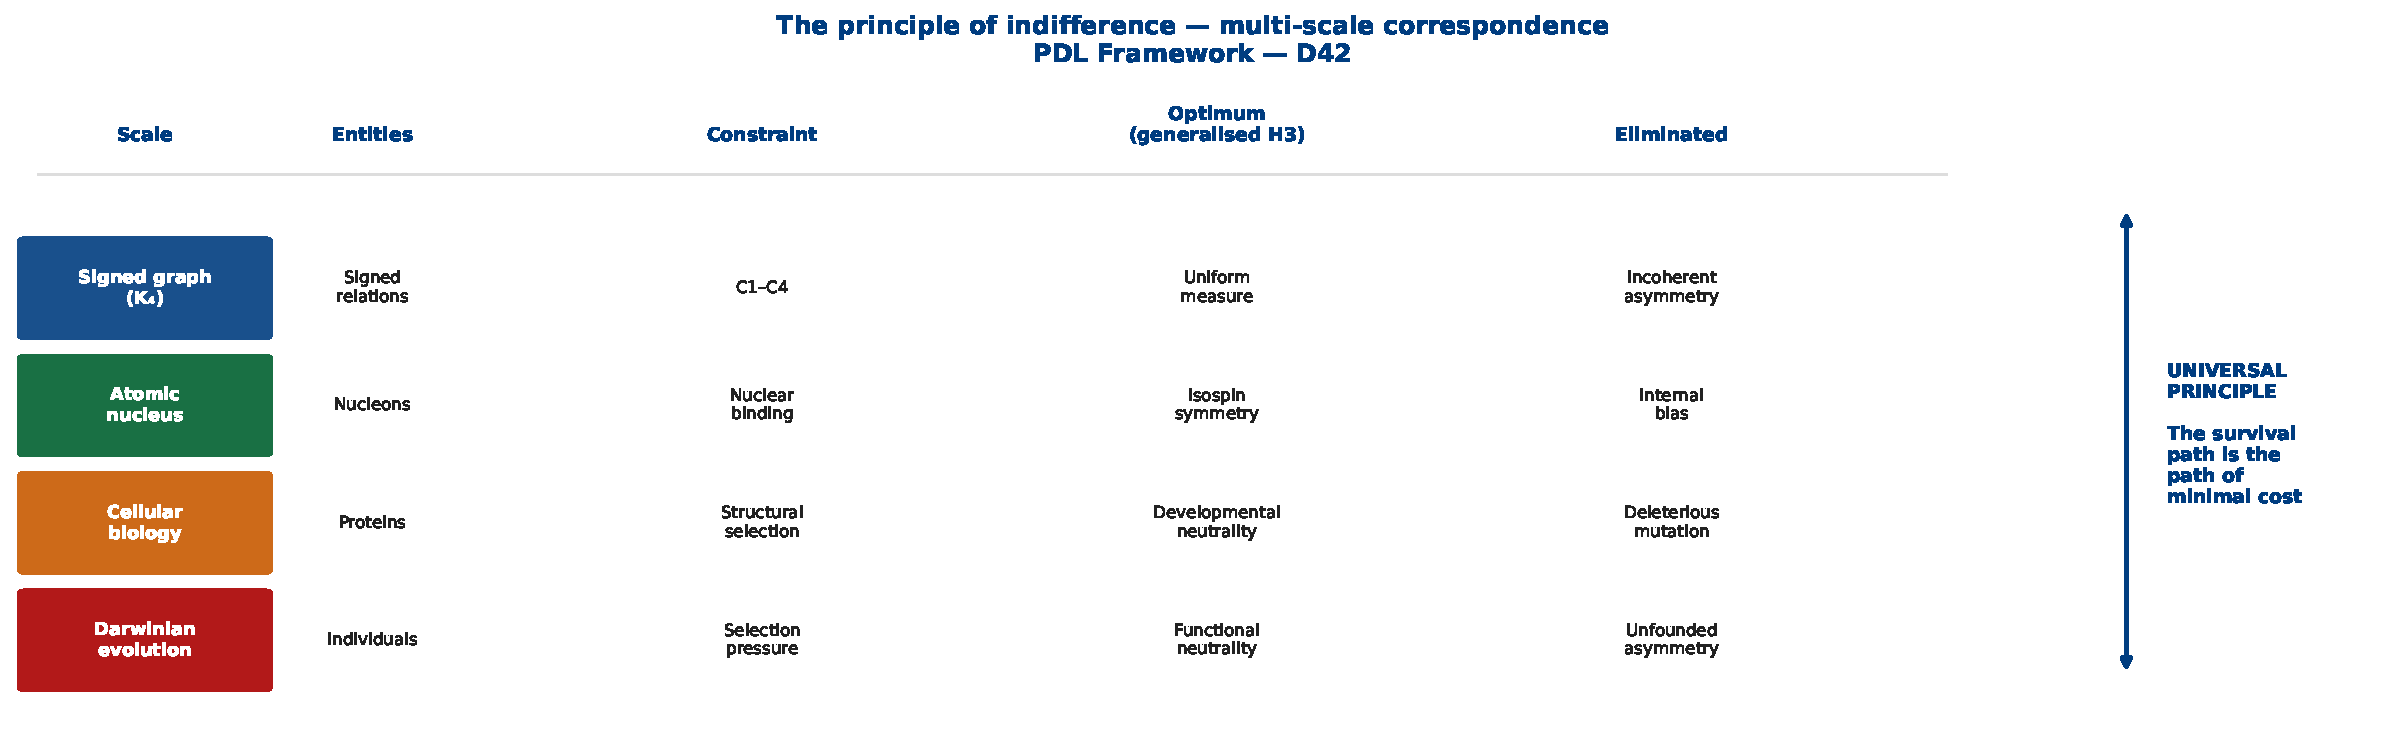
\includegraphics[width=\textwidth]{D42_fig3_multiscale_EN.pdf}
\caption{The principle of indifference across scales. In each row, the optimisation constraint (column 3) eliminates structurally ungrounded asymmetries (column 5) and selects a uniform or neutral distribution (column 4). The same logical structure governs signed graphs, nuclear stability, developmental biology, and Darwinian evolution. The survival principle is identical at every level.}
\label{fig:multiscale}
\end{figure}

\noindent The structural correspondence is as follows. In the \PDL\ graphical layer, an asymmetric measure on $\Rtot$ is a cost with no structural basis under~C4 (since $\Kfour$ cannot distinguish relations via cross-triangles); C4 eliminates it, leaving the uniform measure $H_3$. In nuclear physics, an internal asymmetry in the coherent-triangle participation of nucleons would increase the coherence cost; the valley of stability (D40) is the unique minimum of this cost. In Darwinian evolution, a heritable asymmetry that does not increase reproductive fitness is a cost without return; selection pressure eliminates it, leaving the neutrally optimal genotype. The principle is one: \emph{the survival path is the path of minimal cost, and any asymmetry without structural foundation is a cost}.

This correspondence is not merely analogical. The \PDL\ derivation of nuclear stability (D40~\cite{PDL_D40_2026}) proceeds by the same combinatorial optimisation that yields $H_3$. The valley of stability is derived from the proton quintuplet without free parameters, using the same C4-optimality argument. The multi-scale principle is therefore a theorem of the framework at each level where the framework applies.

% ============================================================
\section{Epistemic status}
\label{sec:status}

\begin{table}[H]
\centering
\caption{Epistemic status of the principal results.}
\label{tab:status}
\begin{tabular}{lll}
\toprule
Result & Status & Dependencies \\
\midrule
Equiparticipation Lemma (D42-L1) & Theorem & C4-optimality, graph theory \\
Cross-triangle blindness (D42-L2) & Theorem (direct, D29~\cite{PDL_D29_2026}) & Definition of $(A)\wedge(B)$ \\
$S_4$-invariance of cross-triangles (D42-L2) & Theorem & $\mathrm{Aut}(K_4)=S_4$, C1--C4 \\
$S_4$-equivariance of cross-edges (D42-L3) & \textbf{Theorem} & Bijectivity of $S_4$, C1--C4 \\
$H_3$ (Indifference Lemma) & \textbf{Theorem} & C1--C4, D16a, D29 \\
$\kap = 310\vp/11017$ & \textbf{Unconditional theorem} & $H_3$ (proved), D05, D29 \\
Causal closure & Corollary + interpretation & Full corpus \\
\bottomrule
\end{tabular}
\end{table}

% ============================================================
\section{Open problems}
\label{sec:open}

The resolution of~OP1~(D39) removes the sole foundational hypothesis from the programme. The remaining open problems are at higher levels of derivation.

\begin{openproblem}[OP12 / BH-3]
Derive the Bekenstein--Hawking formula $S_{\mathrm{BH}} = k_B c^3 A / (4G\hbar)$ from axioms~C1--C4 alone, without invoking the Schwarzschild metric as input.
\end{openproblem}

\begin{openproblem}[OP14]
Derive the sub-shell filling sequence $r_{\mathrm{exc}}(Z) \in \{0,1,2,3\}$ (D40) analytically from~C1--C4. This problem is structurally equivalent to~OP12: both reduce to counting coherent configurations on a collective \PDL\ surface.
\end{openproblem}

\begin{openproblem}[Global uniqueness of the proton quintuplet]
Establish that $(24, 28, 930, 10087,$ $11017)$ is the \emph{globally} unique admissible quintuplet (local uniqueness is proved in~D16b~\cite{PDL_D16b_2026}).
\end{openproblem}

\clearpage
% ============================================================
\bibliographystyle{unsrt}
\bibliography{D42v2_references}

\end{document}